%% -*- mode: poly-noweb+R; ess-indent-level: 2; -*-
\chapter{Az \code{Rxls} csomag felhasználói szemmel}
\label{chap:4}

Az \code{Rxls} csomag exportált függvényei közül valószínűleg azok a
legfontosabbak, melyek segítségével adatokat lehet
\code{EXCEL}-be írni ill. onnan beolvasni. Egy másik csoport a futási 
állapot kiírásával kapcsolatos. Végül van néhány segédfüggvény is.

\section{Adat-átviteli függvények}\label{sec:4.1}
Ezeket a rutinokat már nagyrészt láttuk \aref{sec:1.3} %az 1.3 
részben.

\begin{description}
\item[\code{XLdata}, \code{XLsource}] 
  Az \code{XLdata} függvény segítségével megfelelően
  formázott \code{EXCEL} munkalapról lehet adatokat átvenni. Az \code{XLsource}
  függvény \code{EXCEL}-ben tárolt \code{R kódlap}ot olvas be és értékel ki.
\item[\code{XLreaddf.rows}, \code{XLreaddf.cols}, \code{XLwritedf}] 
  Az \code{XLreaddf.cols} rutin egy
  \code{EXCEL} táblázatot olvas be \code{R}-be. Alapértelmezésben a
  legfelső sor az
  \code{R} oldalon létrehozott \code{data.frame}  neveit adja. Az
  \code{XLreaddf.rows} 
  hasonló, de az \code{EXCEL} táblázatot először transzponáljuk,  azaz az
  első oszlopban vannak a \code{data.frame} nevei, stb. Az
  \code{XLwritedf} függvény 
  egy \code{R} \code{data.frame}-t ír az \code{EXCEL} megadott
  tartományába. A rutin 
  külön figyel a \code{dátum} és \code{factor} típusú adatokra. Az
  \code{NA} értékek üres 
  cellaként jelennek meg. Lehetőség van az  oszlop szélesség
  automatikus beállítására (\code{autoFit} argumentum) és a kitöltött
  tartománynak (munkafüzet szintű) nevet adhatunk (\code{setname}
  argumentum).  
\item[\code{XLget}] A megadott \code{EXCEL} tartomány tartalmát adja
  vissza. Közvetlenül valószínűleg ritkán  lesz rá szükség.

\item[\code{getFromDB}, \code{ACCESS.get}, \code{ODBC.get}]
  \code{ODBC} kapcsolaton keresztül olvas be
  adatokat. A \code{getFromDB} a másik két függvény között választ a
  paramétereitől függgően.
\end{description}

\section{Futási állapot kiírása}\label{sec:4.2}

Itt az elképzelés az, hogy az \code{R} grafikus eszközéhez hasonlóan
van egy \code{logDevice}. Amikor 
az \code{Rxls} csomag betöltődik akkor létrejön az 1-es számú ilyen
eszköz, ami egy \code{null} eszköz. 
Nevéhez méltóan ez semmit nem jelenít meg. A lehetséges
\code{logDevice} típusok \code{null}, \code{R}, \code{EXCEL},
\code{TCL}.

\begin{description}
\item[\code{logDev}, \code{logDev.set}, \code{logDev.off},
  \code{logDev.list}]
  A \code{logDev} függvény új
  \code{logDevice}-t hoz létre a megadott típussal. A
  \code{logDev.set} függvény az 
  aktuális \code{logDevice}-t állítja át, \code{logDev.off}
  kikapcsolja azt, míg a 
  \code{logDev.list} kilistázza a létező \code{logDevice}-okat.  
\item[\code{XLwith}] Ideiglenesen csatolja a keresési úthoz a
  \code{THISXL}(hivatkozás az indító \code{EXCEL} példányra),
  \code{.wbname} (munkafüzetnév), \code{.wsname} (munkalapnév)
  vátozókat és a 
  megadott kifejezést (alapértelmezésben \code{eval(.FUN)})
  végrehajtja (kiértékeli) a munkafüzet saját \code{R} környezetében
  oly módon, hogy a  \code{warning} és \code{stop} \code{message}
  függvények a megadott  típusú \code{logDevice}-ra is írnak.   
\item[\code{background}] A
  megadott kifejezést végrehajtja (kiértékeli) oly módon, hogy a
  \code{warning} és \code{stop} \code{message} függvények a megadott
  típusú \code{logDevice}-ra is 
  írnak.  A különbség az \code{XLwith} függvényhez képest az, hogy a
  globális környezetben történik a kiértékelés és ennek megfelelően
  nem történik meg a fenti változók ideiglenes csatolása a keresési úthoz.
\item[\code{progress}] Egyszerű, szöveges \code{progreszbár}t hoz létre, ami az
  aktuális \code{logDevice}-ra ír. 

\item[\code{logInit}] A \code{logDev} függvény használja. Csak
  kompatibilitási okok miatt maradt az exportált függvények között.
  
\item[\code{logMessage}] A \code{logDevice}-ra ír
  üzenetet. Valószínűleg sohasem kell közvetlenül meghívni.
\end{description}

\section{Segéd függvények}\label{sec:4.3}

\begin{description}
\item[\code{XLDate}, \code{XLPOSIXct}] Ezt függvényt már láttuk
  \aref{sec:1.2} %a 1.2 
  szakasz
  végén. Ha \code{XLreaddf} függvényeket használjuk, akkor az eredményben a
  dátum típusú adatok számként jelennek meg.  Ez a függvény a számokat
  az \code{R} \code{Date} típusú adatává alakítja. Tisztában kell azonban lenni
  azzal, hogy más dátum típusok is léteznek \code{R}-ben: \code{POSIXct} és
  \code{POSIXlt}. Ha ilyen típusú adatra van szükségünk, akkor használjuk az
  \code{as.POSIXct} és \code{as.POSIXlt} függvényeket.  

  További lehetőség, hogy az
  \code{XLreaddf} függvényeket \code{value="value"} argumentummal
  hívjuk meg. Ezt 
  nem tartom megbízható megoldásnak. Tapasztalatom szerint a nyári
  időszámítás miatt egy napos eltolódás előfordulhat a dátum típusú 
  adatoknál. Az ok, valahol az időzóna és a nyári időszámítás
  kezelésében lehet.  
  \begin{Rnw}
<<echo=FALSE,results="hide">>=
getExcelWithRdev()
withObj(THISXL,.[["visible"]]<-TRUE)
ActiveCellInNewWb()
THISXL$run("R.RIC.connect",TRUE)
@ 
<<>>=
x<-seq.Date(as.Date ("2013-01-01"),as.Date ("2014-01-1"),by="1 month")
df<-data.frame(date=x)
XLwritedf(df=df,setname="datumok")
df["R->EXCEL->R.date"]<-XLreaddf.cols("datumok",value="value")
df["eltérés"]<-with(df,as.POSIXct(as.POSIXlt(date),tz="CET")-`R->EXCEL->R.date`)
df["eltérés2"]<-with(df,date-as.Date(`R->EXCEL->R.date`,tz=""))
df[with (df,`eltérés`!=0 | `eltérés2`!=0),,drop=FALSE]
@ 
  \end{Rnw}
 % > x <- seq.Date(as.Date("2013-01-01"),
 %  as.Date("2014-01-1"), + by = "1 month") > df <- data.frame(date = x)
 %  > XLwritedf(df = df, setname = "datumok") NULL >
 %  df["R->EXCEL->R.date"] <- XLreaddf.cols("datumok", value = "value")
 %  > df date R->EXCEL->R.date 1 2013-01-01 2012-12-31 23:00:00 2
 %  2013-02-01 2013-02-01 00:00:00 3 2013-03-01 2013-03-01 00:00:00 4
 %  2013-04-01 2013-04-01 01:00:00 5 2013-05-01 2013-05-01 00:00:00 6
 %  2013-06-01 2013-06-01 00:00:00 7 2013-07-01 2013-07-01 00:00:00 8
 %  2013-08-01 2013-08-01 00:00:00 9 2013-09-01 2013-09-01 00:00:00 10
 %  2013-10-01 2013-10-01 00:00:00 11 2013-11-01 2013-10-31 23:00:00 12
 %  2013-12-01 2013-12-01 00:00:00 13 2014-01-01 2014-01-01 00:00:00
  Külön bosszantó, hogy az eredmény még attól is függ, hogyan olvassuk
  ki az adatokat.  Mást kaphatunk, ha csupa dátum típusú adatot
  tartalmazó tartományt olvasunk be, és mást akkor ha csak néhány
  cella dátum típusú.  
  \begin{Rnw}
<<>>=
x1<-XLget("datumok")[2:14,1]
x1<-Rxls:::unlist.keepclass(x1)
x2<-XLget(XLrange=THISXL$range("datumok")$range("A2:A14"))
x2<-Rxls:::unlist.keepclass(x2)
df<-data.frame("név cellával"=x1,
               "név cella nélkül"= x2, "eltérés"=x1-x2,
               check.names=FALSE)
df[with(df,`eltérés`!=0),]
@ 
  \end{Rnw}
% > x1 <- XLget("datumok")[2:14, 1] > x2 <-
%   XLget(XLrange = THISXL$range("datumok")$range("A2:A14")) >
%   data.frame(‘név cellával‘ = Rxls:::unlist.keepclass(x1), + ‘név
%   cella nélkül‘ = Rxls:::unlist.keepclass(x2), check.names = FALSE)
%   név cellával név cella nélkül 1 2012-12-31 23:00:00 2012-12-31
%   23:00:00 2 2013-02-01 00:00:00 2013-01-31 23:00:00 20
%   2013-03-01 2013-04-01 2013-05-01 2013-06-01 2013-07-01 2013-08-01
%   2013-09-01 2013-10-01 2013-10-31 2013-12-01 2014-01-01
%   00:00:00 01:00:00 00:00:00 00:00:00 00:00:00 00:00:00 00:00:00
%   00:00:00 23:00:00 00:00:00 00:00:00
%   2013-02-28 2013-04-01 2013-05-01 2013-06-01 2013-07-01 2013-08-01
%   2013-09-01 2013-10-01 2013-10-31 2013-11-30 2013-12-31
%   23:00:00 00:00:00 00:00:00 00:00:00 00:00:00 00:00:00 00:00:00
%   00:00:00 23:00:00 23:00:00 23:00:00
  Emellett az 1970 előtti dátumok kezelése is problémás a \code{value}
  tulajdonság használata esetén. Összefoglalva a \code{"value2"}
  tulajdonság használatát javaslom, a dátum értékek utólagos
  transzformációjával az \code{XLDate} vagy az \code{XLPOSIXct}
  függvényekkel. Utóbbi \code{POSIXct} formátumba alakítja az adatot, amivel
  a napon belüli időpont sem veszik el.  
\item[\code{XLScreenUpdateTurnOff}] Az
  \code{XLwritedf} rutin használja, de egyéb esetekben is szükség lehet rá,
  ha nagy mennyiségű adatot írunk \code{EXCEL} munkalapra. Kikapcsolja az
  \code{EXCEL} képernyő frissítését és a kalkuláció módját kézire
  állítja. Ez utóbbi azt jelenti, hogy az adatok írása nem fogja az
  érintett cellák újraszámolását triggerelni. Visszatérési értéke egy
  függvény, ami visszaállítja az eredeti állapotot. Tipikus
  használata:
  \begin{Rnw}
<<eval=FALSE,prompt=FALSE>>=
turnOn <- XLScreenUpdateTurnOff(Appl = THISXL)
on.exit(turnOn(), add = TRUE)
@ 
\end{Rnw} 

\item[\code{XLusedrange}] A (\code{COMObject} formában)
  megadott tartománynak és a tartomány munkalapján érvényes
  \code{usedrange}-nek a metszetét számolja ki. 
  Akkor van jelentősége, ha pl. szeretnénk a \code{\$A:\$A}
  oszlop elemeit beolvasni R-be. A természetesnek tűnő
  \begin{Rnw}
<<eval=FALSE,prompt=FALSE>>=
THISXL$range("$A:$A")$value()  
@ 
  \end{Rnw}
  hívás eredménye egy olyan mátrix, aminek annyi sora van, ahány az
  \code{EXCEL} munkalapnak. Ez 32-bites OFFICE esetén is túl sok, 64-bites
  OFFICE esetén pedig több mint 1 millió sort jelent. Ezt valószínűleg
  úgy élnénk meg, hogy lefagyott a program, holott  csak nagy
  mennyiségű adatot másol meglehetősen lassan. 
\item[\code{.XLrange}] Szöveges címből állít elő hivatkozást
  (\code{COMObject}). A cím lehet teljes külső cím, munkafüzettel és
  munkalappal, vagy a tartomány \code{EXCEL}ben definiált neve. Ha
  lehet célszerű a tartományokra névvel hivatkozni. 
\item[\code{attachXL}] Csatolja a \code{THISXL, .wbname, .wsname}
  változókat a keresési úthoz. A visszatérési érték egy függvény amit
  a csatolás megszüntetésére lehet használni. Pl. az \code{XLwith}
  függvény elese a következő
  \begin{Rnw}
<<eval=FALSE,prompt=FALSE>>=
detachXL<-attachXL(env)
on.exit(detachXL(),add=TRUE)
@     
  \end{Rnw}
  Itt \code{env} a munkafüzet \code{R} környezete. Ez automatikusan
  létrejön amikor az \code{EXCEL} csatlakozik az \code{R}-hez.

\item[\code{withXLenv}] Hasonló az \code{R} \code{with} függvényéhez,
    bár az argumentumok sorrendje éppen fordított. Kiértékel egy
    \code{R} kifejezést a megadott környezetben. Ha a környezet nincs
    megadva, de csak egy csatlakoztatott munkafüzet van, akkor annak a
    környezetét használja a rutin. Tesztelés során lehet hasznos.

\item[\code{detachXLenvs}] Eltávolítja a keresési útvonalról
  valamennyi \code{EXCEL} környezetet. 

\item[\code{win.stop}] A \code{stop}
  függvényhez hasonlóan leállítja a futást, de a hiba üzenet nem csak
  az \code{R} konzolban, hanem egy felugró ablakban is megjelenik.  
\item[\code{pkgzip}] A
  megadott és telepített \code{R} csomagokat becsomagolja \code{win-binary}
  formátumba.  
\item[\code{installRxls}] Az \code{Rxls} csomagban lévő \code{EXCEL} fileokat
  másolja az \code{\{APPDATA\}/Rxls} könyvtárba. Emellett ide kerül még egy
  \code{versions} nevű file is, ami a verzió információt tartalmazza.
\item[\code{getHWND}] Az \code{R} konzol ablakának azonosítóját adja
  vissza. Az új \code{R.xls} 
  munkafüzet nem használja.  
\item[\code{install.xls}] Az \code{R.xls}-t használó
  munkafüzetek telepítője. Az adott csomag \code{EXCEL} könyvtárában lévő
  \code{EXCEL} file-okat a kiválasztott könyvtárba másolja és beállítja az
  \code{R.xls}-re  történő hivatkozást. Az új számolómunkafüzetekhez
  nincs rá szükség.
\item[\code{R\_RegEntries}] Az \code{R}-rel kapcsolatos
  regisztry bejegyzéseket jeleníti meg.  
\end{description}

\section{A background és logDev függvény
  részletesebben}\label{sec:4.4}

A munkafüzet tipikusan tartalmaz egy gombot, mellyel a felhasználó a
számolást elindítja. A gomb makró-hozzárendelése lehet
\code{cmdbtnHosszufutas} vagy \code{cmdbtnRovidFutas}. Ha a 
gombot a \code{Cella menü -> Insert Form -> Run button} paranccsal
hoztuk létre, akkor áttételesen de a \code{cmdbtnHosszufutas} szubrutint
használjuk. Ezek részletes ismertetését lásd \aref{sec:5.3} %a 5.3 
szakaszban. Mindkét rutin megkeresi a végrehajtandó kódot. Ez
jellemzően a gomb alatti cellából derül ki. A kód egy szöveg. Ezt
célszerű munkalap függvényeket használva összerakni 
valamelyik \code{R kód(<név>)} munkalapon. Ezt a szöveget, mint a \code{.FUN}
szimbólum definícióját 
átadjuk az \code{R} szervernek. Pl. ha az \code{EXCEL}-ben kiszámolt
kód:
\begin{Rnw}
<<echo=FALSE,results="hide">>=
txt<-c("print('Ez egy üzenet EXCELből');",
       "withObj(THISXL[['activecell']][['offset',1]],.[['value']]<-'Ez meg a válasz')")
THISXL
wb<-THISXL$workbooks()$add()
wb$activate()
THISXL$range("$A$1")$activate()
withObj(THISXL$activecell(),{
            .[["value"]]<-paste(txt,collapse=" ")
            .[["wraptext"]]<-FALSE
            .$entirecolumn()$autofit()
        })
THISXL$run("Rdev.xlam!insertform.insertcalcbtn",", short:=True")
Sys.sleep(.5)
cmd<-THISXL$activesheet()$shapes(1)$onaction()
Sys.sleep(.5)
suppressMessages(THISXL$run(cmd))
Sys.sleep(.5)
withObj(THISXL,.[["height"]]<-130)
capturewnd("FUN_result.bmp")
wb<-NULL
gc()
cmd<-change.cmd(THISXL$run("R.RIC.defaultcmd"),
                fun="with",
                keep=c(data="env"),
                expr=substitute (.FUN))
                                        #$ 
@ 

<<echo=FALSE>>=
cat(paste(txt,collapse="\n"))
@ 
\end{Rnw}

Akkor a gomb megnyomása után az R oldalon a \code{.FUN} szimbólum értéke a
következő:
\begin{Rnw}
<<code=cmd>>=
@  
\end{Rnw}
A \code{.FUN} változó értékadásához %Ebben a lépésben 
az \code{R} oldal \code{COM} interfészét használjuk.
\begin{figure}[h]
  \centering
  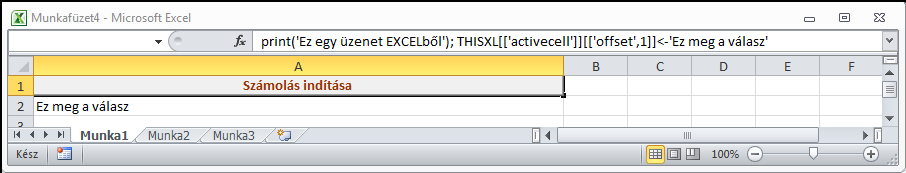
\includegraphics{images/FUN_result}
  \caption{A munkalap képe a számolás gomb megnyomása után. A gomb
    alatti cellában található a végrehajtandó R kód.}
  \label{fig:4.1}
\end{figure}

%4.1. ábra. 
A következő lépésben a kódot végre kell hajtani. Attól függően járunk
el, hogy a várható 
futási idő rövid (\code{cmdbtnRovidfutas}), vagy hosszú (\code{cmdbtnHosszuFutas}). Az első esetben a
végrehajtáshoz is használhatjuk a \code{COM} interfészt, azonban a
második esetben aszinkron hívásra van szükségünk. Ennek az az oka,
hogy ellenkező esetben az \code{EXCEL} nem fog reagálni 
a kód futása alatt, ráadásul az \code{EXCEL} rendszeres időközönként
megjelenít egy figyelmeztető
ablakot, miszerint az \code{EXCEL} ole művelet befejezésére vár. 
Ebben az állapotban kilépni sem
lehet az \code{EXCEL}-ből.


Az aszinkron függvényhívás jelenleg nagyon egyszerűen van megoldva. A
kapcsolat inicializálásakor, lekérdezzük az \code{R} ablak számát
(\code{window handle}) és ennek az ablaknak elküldjük a
\code{XLwith(env=<XL környezet>)}\footnote{Ez egy változás a 2.0.250
  verzióhoz képest. Ha azt a hibaüzenetet tatpasztaljuk, hogy a
  rendszer nem találja a  \code{background} függvényt, akkor
  frissíteni kell az \code{Rxls} csomagot a legújabb változatra. Egyéb
tekintetben a korábbi változatokkal készített számoló munkafüzeteknek
elvben működnie kell az új \code{Rxls} csomaggal.} szöveget a Windows
üzenet küldési mechanizmusával. Ezt 
az \code{R} úgy érzékeli, mintha a felhasználó beírta volna a konzolba
(akkor is, ha egyébként az \code{R} ablak el van rejtve) és a kapott
kifejezést kiértékeli. Ez a megoldás eddig megbízhatóan működött, de
nyilvánvaló, hogy hosszútávon célszerű lenne kiváltani a megfelelő
\code{COM} mechanizmussal.  

Megjegyzendő, hogy az
\code{Rstudio} 
használata esetén ez a megoldás nem alkalmazható, mert ez az
alkalmazás a kapott üzenetet 
nem írja be az \code{R} konzolba, ezért \code{Rstudio} ill. terminál
ablakban futtatott \code{R} esetén a \code{sendkeys} 
függvényt használjuk.

Az \code{XLwith} függvény definíciója a következő:
\begin{Rnw}
<<>>=
XLwith
@ 
\end{Rnw}
Azaz az \code{expr} \code{R} kifejezést kiértékeljük, de speciális
környezetben. Ha a kifejezés kiértékelése közben, hiba, figyelmeztetés
vagy üzenet keletkezik az nem csak az R ablakban, hanem 
az aktuális \code{logDevice}-on is megjelenik. Jelenleg a működés
hasonló a rajz felületek (\code{graphical devices}) kezeléséhez. A
\code{logDev} függvény segítségével hozhatunk létre új eszközt, a 
\code{logDev.off} törli az aktív eszközt, a \code{logDev.set} pedig
átállítja az aktuális eszközt. Jelenleg 
négy féle eszköz áll rendelkezésre: \code{null}, \code{EXCEL},
\code{TCL} és \code{R}.

A \code{null device} nevéhez méltóan nem add semmit az \code{R} beépített
mechanizmusához. Az 
\code{EXCEL} \code{logDevice} az \code{EXCEL} státuszbárjában jeleníti
meg az üzeneteket. A \code{TCL} eszköz megjelenít egy ablakot és ezt
használja, míg a \code{R} eszköz az \code{R} konzolját használja. 

A \code{logDevice} eszköz létrehozásakor az volt a cél, hogy
egyszerűen lehessen a futási 
állapotot megjeleníteni, lehetőleg anélkül, hogy a kódot teletűzdelnénk
\begin{verbatim}
THISXL[["statusbar"]]<-"...";...;THISXL[["statusbar"]]<-FALSE
\end{verbatim}
párokkal. % teletuzdelni.

\paragraph{Megjegyzés.} A \code{logDevice} elgondolás fokozatosan
született meg. A korábban született alkalmazások, vagy közvetlenül
használják az \code{EXCEL} státuszsorát, vagy a fent leírt megoldás 
előzetes változatát. A később született alkalmazásokban megjelent a
\code{logInit} függvény használata. Ez még nem a fent leírt \code{log}
eszköz. A \code{logInit} függvény egy olyan objektumot hozott 
létre, amivel vagy az \code{EXCEL} státusz sorában vagy egy \code{TCL}
ablakban lehetett szöveges üzenetet 
ill. \code{progressbar}-t megjeleníteni. Jelenleg már az \code{R}-ben
is elérhető a \code{txtProgressBar} ill. a 
\code{winProgressBar} függvény.

%\begin{Rnw}
%<<>>=
%XLwith
%attachXL
%detachXLenvs
%@ 
%\end{Rnw}


\section{A \code{progress} függvény használata}\label{sec:4.5}

Az a tapasztalatom, hogy egy számolás elindítása után, ha a
felhasználó nem kap visszajelzést, hogy valami történik, akkor rövid
időn belül elkezdi nyomkodni a billentyűzetet, klikkelget, a
jártasabbak pedig a feladatkezelőn keresztül kilövik a programot,
hiszen az nem csinál semmit. Ha a számolást \code{EXCEL}-ből
indítottuk a legkézenfekvőbb az \code{EXCEL} státuszbárjában
megjeleníteni a számolás aktuális állását. Ezt legegyszerűbben úgy
érhetjük el, hogy 
az előző pontban ismertetett \code{logDev("EXCEL")} függvényhívást
használjuk. Tesztelés során 
hasznos lehet a \code{logDev("R")}, vagy \code{logDev("TCL")} is.

A \code{progress} függvény egy új \code{progressbar}-t hoz létre az
aktuális \code{logDevice}-on. Tegyük 
fel, hogy a számolás különböző fázisai az adatok beolvasása \code{ACCESS}ből, számolás, majd az
eredmények mentése. Ekkor a végrehajtandó (meta) kód a következő képpen alakul.
\begin{Rnw}
<<eval=FALSE,prompt=FALSE>>=
data <- read.access()
res <- do.calc(data)
save.results(res)
@ 
\end{Rnw}
Ha szeretnénk a felhasználót tájékoztatni az egyes fázisokról, akkor ez kiegészül a következőképpen
\begin{Rnw}
<<eval=FALSE,prompt=FALSE>>=
pb <- progress("%s...", "")
pb$step("ACCESS adatbázis olvasása")
data <- read.access()
pb$step("Számolás")
res <- do.calc(data)
pb$step("Eredmények mentése")
save.results(res)
pb$rm()
rm(pb)
@ 
\end{Rnw}
Tegyük fel, hogy a számolás hosszú, mondjuk a beolvasott adatok
mindegyikén el kell 
végezni egy műveletet, ami maga is időigényes. Ekkor a \code{do.calc}
függvény szerkezete a következő lehet
\begin{Rnw}
<<eval=FALSE,prompt=FALSE>>=
do.calc <- function(x) {
    pb <- progress(sprintf(" [%%d/%d]", length(x)), 0, lazyness = 0.3)
    on.exit({
        pb$refresh()
        pb$rm()
    })
    sapply(x, function(y) {
               pb$inc()
               ## egy számolási lépés y-on
           })
}
@ 
\end{Rnw}
A függvény első sorában létrehozunk egy \code{progressbar}-t. A
\code{progress} függvény első argumentuma egy minta, ami jelen esetben
az \code{x} vektor hosszától függ. Ha pl. \code{length (x) = 
100}, akkor a minta (\code{pattern}) értéke \code{" [\%d/100]"} lesz. A mintában szereplő \code{\%d} helyére egy
egész érték kerül, aminek kezdőértéke 0, ez a második argumentum.

A \code{lazyness} paraméter a megjelenítés sűrűségét állítja be. Ha
nem adjuk meg, akkor minden változás után frissítjük a
\code{logDevice}-on látható szöveget. Pozitív \code{lazyness} érték mellett 
csak akkor frissítjük a \code{logDevice}-ot, ha az előző frissítés óta
eltelt idő (másodpercben mérve) 
legalább akkora, mint a \code{lazyness} értéke. A 0.3 másodperces
\code{lazyness} érték mellett a kijelzést 
folyamatosnak érezzük, de nem írunk feleslegesen sokszor a \code{logDevice}-ra.
A függvényből való kilépéskor frissítjük a \code{logDevice} szövegét,
majd töröljük az eszközről a \code{pb} \code{progressbar}-t. Magát a
\code{pb} változót  nem kell törölnünk, mivel a függvényből való
kilépéskor megszűnik az a környezet, amiben definiáltuk.

Amikor a \code{pb\$inc()} hívást végrehajtjuk, akkor a
\code{progressbar}-ban tárolt értéket eggyel 
növeljük és megpróbáljuk frissíteni a \code{logDevice} szövegét. Ez
csak akkor fog megtörténni, ha 
az előző frissítés óta eltelt idő nagyobb mint a \code{lazyness}
érték. Emiatt a kijelző nem folyamatosan számol. Ezért került az
\code{on.exit} rutin elejére egy extra frissítés. Így nem fordulhat elő, 
hogy a számláló ,,elakad'' 98-nál.

A fenti mintakód esetén a számolás szakaszban a \code{logDevice}
szövege az alábbihoz hasonló: 
\begin{verbatim}
Számolás... [23/100]
\end{verbatim}
A \code{Számolás...} szövegrész a globálisan használt progressbar
értéke, míg a \code{ [23/100]} a 
\code{do.calc} függvény járuléka.

Gyakran nem a \code{inc}, hanem a \code{step} metódust alkalmazzuk egy
\code{progressbar}nál. Ekkor a 
\code{logDevice}-on megjelenített szöveg a
\begin{verbatim}
sprintf(pattern,...)
\end{verbatim}
függvényhívás eredménye, ahol a \code{pattern} az inicializáláskor vagy a
\code{reset} metódus hívásakor megadott minta, \code{...} pedig a
\code{step} hívás argumentumait jelöli. 

\endinput

%%% Local Variables: 
%%% mode: latex
%%% TeX-master: "Rxls"
%%% End: 
